\chapter{Code Generation from the ProPCPN DYMO Model}
\label{chap:dymo}
The producer-consumer system, we have focused on until now, is a small ProPCPN model created to illustrate the basic concepts. In this chapter we describe how code is generated from a ProPCPN model of the Dynamic MANET On-demand (DYMO) routing protocol, which is an advanced industrial-sized communication protocol. The DYMO protocol is introduced in section~\ref{sec:dymooverview}. In section~\ref{sec:dymomodel} we present a ProPCPN model of the DYMO protocol which contains more advanced modelling constructs than the producer-consumer ProPCPN model. In section~\ref{sec:dymoexperiments} we describe and validate the code generated from the DYMO model. 

\section{The DYMO Protocol}
\label{sec:dymooverview}
The Dynamic MANET On-demand routing protocol is a routing protocol for \emph{mobile ad-hoc networks} (MANETs). It is currently under development by the IETF MANET working group \cite{RefWorks:89}. The specification is an Internet-draft \cite{RefWorks:88}, and is expected to become a Request for Comments (RFC) document in the near future.

\subsection{Mobile Ad-hoc Networks}
A MANET \cite{RefWorks:90} is a network consisting of mobile nodes, e.g., laptops, or mobile phones. The network has no pre-existing communication infrastructure in contrast to, e.g., WLANs where the nodes communicate with each other through a base station. The nodes in a MANET must therefore communicate directly with one another, i.e., send messages to those nodes that are within physical transmission range. This means, that it is the power of the radio, and the physical position of the nodes, that determine the topology of the network. The topology of the network may change rapidly because of node mobility, and links between nodes might disappear and reappear frequently. A typical use of MANETs is during emergency search-and-rescue operations in remote areas where no pre-existing communication infrastructure exists. 

\newpage

In order to communicate with nodes outside a given nodes physical range a routing protocol is needed to perform multi-hop communication, i.e., nodes forward data packets on behalf of other nodes in the network. The topology of a small MANET with five nodes is shown in Fig.~\ref{fig:topology}. An edge between two nodes indicates that the nodes are within direct transmission range of each other, e.g., node 1 is able to send messages directly to node 2 and node 3. 

\begin{figure}
\centering
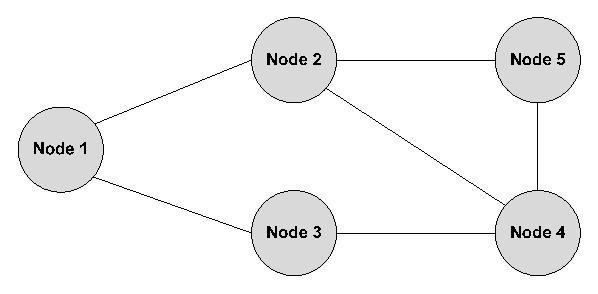
\includegraphics[scale=0.8]{dymo/graphics/topology_ex.eps}
\caption{Five node example topology}
\label{fig:topology}
\end{figure}

Routing protocols for MANETs are often categorised as being either \emph{proactive} or \emph{reactive}. The proactive routing protocols are constantly trying to keep an updated view of the network topology by maintaining a route to the other nodes in the network. The reactive routing protocols establish routes on demand, i.e., when routes are needed, and often do little maintenance on existing routes.

\subsection{The Operations of DYMO}
The DYMO routing protocol is a reactive protocol which establishes routes only when they are needed. The protocol has two main parts which are \emph{route discovery} and \emph{route maintenance}. Route maintenance is done by using active link monitoring and timeouts. If a node becomes aware that a route is broken it sends a \emph{Route Error} (RERR) message to the surrounding nodes, and thereby informs them that the route can no longer be used.

Route discovery is used to establish routes to other nodes in the network. An \emph{originator} node multicasts a \emph{Route Request} (RREQ) message which is sent hop-by-hop throughout the network to find a route to the \emph{target} node of the request. Each intermediate node records a route back to the originator node. When the target node receives the RREQ message it replies with a \emph{Route Reply} (RREP) message. This is unicasted back hop-by-hop towards the originator node using the routes recorded when the RREQ was sent. When the originator node receives the RREP message, the route has been established between the originator node and the target node in both directions.


\begin{figure}
\centering
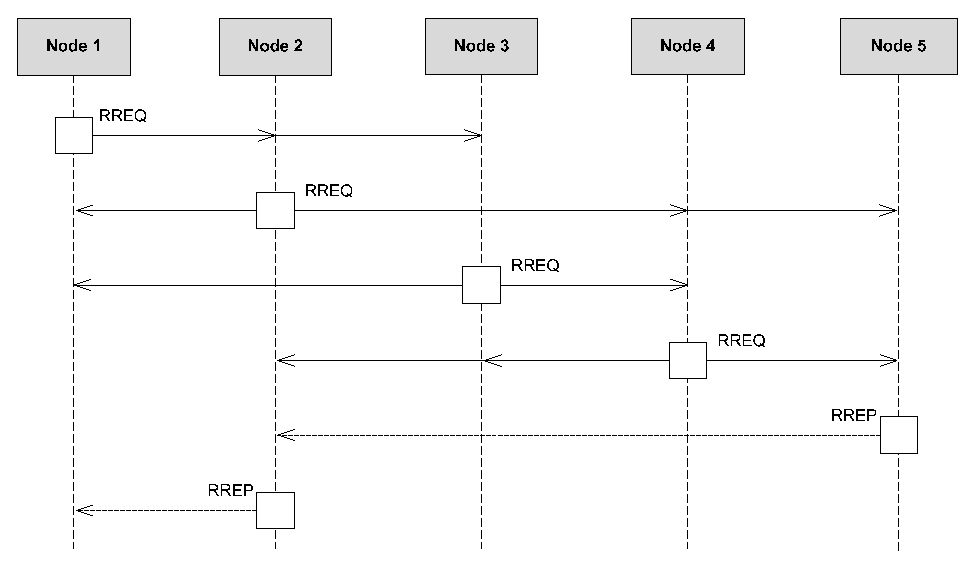
\includegraphics[width=\textwidth]{dymo/graphics/mscdymoex.eps}
\caption{Message sequence chart of a route request}
\label{fig:mscrreq}
\end{figure}

To get a better understanding of the protocol we present an example of how route discovery is performed in the small MANET shown in Fig.~\ref{fig:topology}. Fig.~\ref{fig:mscrreq} shows a message sequence chart (MSC) of one possible exchange of messages in the DYMO protocol when the originator node 1 is requesting a route to the target node 5. A solid arc represents multicast, and a dashed arc represents unicast. In the MSC, node 1 initiates the route request by multicasting a RREQ which is received by nodes 2 and 3. Node 2 and node 3 both records the route back to node 1 in their \emph{routing tables}, and then forwards the RREQ. Node 2 multicasts the RREQ message which is received by the nodes within transmission range, i.e., node 1, node 4, and node 5. Node 3 also multicasts the RREQ message which is received by node 1, and node 4. Node 1 discards the RREQs from node 2 and node 3 because it is the originator of the message. Node 4 first receives the RREQ from node 2 and records the route back to node 1. When node 4 receives the RREQ from node 3, it has already recorded a route to node 1 with the same length (number of hops) and the message is discarded.

Node 4 then multicasts the RREQ which is received by node 2, node 3, and node 5. The message is discarded by node 2 and node 3 since they already know of a shorter route to the originator node 1. Node 5 has received a RREQ from both node 2 and node 4, but since the RREQ from node 2 has a shorter route to node 1 this route is recorded in the routing table. Furthermore, node 5 is the target of the RREQ, and therefore replies with a RREP message with node 1 as the target. The RREP is unicasted back along the same route as the RREQ was sent which means that node 5 sends the RREP to node 2. When node 2 receives the RREP it already knows a route to node 1 (because of the RREQ) and unicasts the RREP to node 1. When node 1 receives the RREP a route is established between node 1 and node 5 in both directions.
\section{Modelling the DYMO Protocol}
\label{sec:dymomodel}

In this section we present the ProPCPN model of the DYMO protocol. The model is constructed on the basis of the DYMO CPN model presented in \cite{RefWorks:6}. The main difference between the model presented in this section, and the model in \cite{RefWorks:6}, is that the control flow of the protocol and access of variables is represented in the structure of the ProPCPN model which is characteristic for the ProPCPN models. The model presented in this section only captures the behaviour of the route discovery part of the protocol. To make the model more readable we present a hierarchical version of the model. Using a hierarchical ProPCPN model do not add expressive power since a hierarchical CPN model (and thus a PropCPN model) can always be transformed to an equivalent non-hierarchical CPN model with the same behaviour (p. 130, \cite{RefWorks:87}). A hierarchical CPN model is organised as a set of hierarchically related \emph{modules}. A module contains places and transitions, and can be seen as a component of the full CPN model.

\subsubsection{The System Module}

\begin{figure}[b!]
\centering
\includegraphics[width=\textwidth]{dymo/graphics/systemmodule.eps}
\caption{The \figitem{System} module of the ProPCPN DYMO model}
\label{fig:dymosystemmodule}
\end{figure}

Fig.~\ref{fig:dymosystemmodule} shows the prime (the root) module \figitem{System} of the ProPCPN DYMO model. The \figitem{System} module contains five \emph{substitution transitions} which are drawn as rectangular boxes with double lines. The substitution transitions are named \figitem{Establishchecker}, \figitem{Initiator}, \figitem{Network}, \figitem{Receiver}, and \figitem{Processer}. Each substitution transition is associated with a module which models the behaviour of the substitution transition. Tokens are exchanged between module using \emph{ports}. The ports constitutes the \emph{interface} of the module, i.e., a module can receive input via \emph{input ports}, and produce output via \emph{output ports}. In Fig.~\ref{fig:dymosystemmodule} all places are \emph{sockets}, i.e., places that are associated with an input or output port. The \figitem{System} module ties together the different parts of the protocol. The \figitem{Initiator} substitution transition creates new route requests. The \figitem{Establishchecker} substitution transition is responsible for notifying when a route has been established. The \figitem{Receiver} substitution transition judges the usefulness of the routing information found in received messages. The routing table is updated with the routing information if it is found useful. The messages that have not been discarded by the \figitem{Receiver} are send to the \figitem{Processer} that processes the messages depending on the message being a request or a reply. When the \figitem{Processer} has processed the message it can forward messages. The \figitem{Network} module is a simple reliable network. It forwards messages which is added to \figitem{DYMOToNetwork} and delivers it to the receiver by adding it to the place \figitem{NetworkToDYMO}.

\subsubsection{The Initiator Module}

\begin{figure}[b!]
\centering
\includegraphics[width=\textwidth]{dymo/graphics/initiatormodule.eps}
\caption{The \figitem{Initiator} module of the ProPCPN DYMO model}
\label{fig:initiatormodule}
\end{figure}

Next, we take a closer look at the \figitem{Initiator} module shown in Fig.~\ref{fig:initiatormodule}. As mentioned this module is responsible for creating route request which is performed by the transition \figitem{CreateRREQ}. To create a route request the transition needs information about its own IP address, the target IP address, and the sequence number to put into the message. The IP address of a node is stored locally at the local place \figitem{OwnIPAddress}. The sequence number and the target IP address, is also used by the \figitem{Processer}, and is therefore modelled as shared places. To avoid too many arcs, which would make the model less readable, we have created shared places using \emph{fusion sets}. Places in different modules belonging to the same fusion set can be seen as one compound place, i.e., they always share the same marking, and they have the same colour set and initial marking.

The transition \figitem{CreateRREQ} do not produce route requests if a route already has been esbablished (determined by the shared place \figitem{RouteEstablished}), the retries limit has been reached (determined by the local place \figitem{RREQ\_TRIES}), or the request has been cancelled (determined by the local place \figitem{Cancel}). When a request has been made it is added to the buffer place \figitem{DYMOToNetwork}. This place has the \emph{output port tag} attached to show that it is an output port. As we saw in the \figitem{System} module in Fig.~\ref{fig:dymosystemmodule}, this place is assigned to a socket place with the same name connected to the \figitem{Network} substitution transition.

The other two transitions in the module handle the cancelation of requests. \figitem{RREQ\_TRIESReached} is enabled when the maximum number of retries has been reached, and it sets the value of the local place \figitem{Cancel} to true. When \figitem{Cancel} is true \figitem{CancelRequest} is enabled which means that no further action should be taken with this request.

\subsubsection{The Processer Module}
\begin{figure}
\centering
\includegraphics[width=\textwidth]{dymo/graphics/processermodule.eps}
\caption{The \figitem{Processer} module of the ProPCPN DYMO model}
\label{fig:processermodule}
\end{figure}

Moving on to Fig.~\ref{fig:processermodule} we find the \figitem{Processer} module. The \figitem{Processer} receives messages from the \figitem{Receiver} on the buffer place \figitem{IncomingMessages}. When a message arrives, the transition \figitem{ReceiveIncomingMessage} becomes enabled, and when it occurs the message is added to the local place \figitem{MessageForProcessing} for further processing. The process token is then added to the process place \figitem{ProcessingMessage}, and the control flow either continues to the substitution transition \figitem{RREPprocesser} or to the substitution transition \figitem{RREQprocesser} (depending on the type of the message).

\subsubsection{The RREPprocesser Module}
\begin{figure}
\centering
\includegraphics[width=\textwidth]{dymo/graphics/rrepprocessermodule.eps}
\caption{The \figitem{RREP processer} module of the ProPCPN DYMO model}
\label{fig:rrepprocessermodule}
\end{figure}

The \figitem{RREPprocesser} module (shown in Fig.~\ref{fig:rrepprocessermodule}) processes incoming messages which has the type RREP, i.e., a route reply. The messages are added to the local place \figitem{MessageForProcessing}, and if the current node is the target, the transition \figitem{RREPTarget} is enabled. An occurrence of \figitem{RREPTarget} means that the route has been established, and by adding the IP address of the originator of the RREP to the buffer place \figitem{NewConnectionEstablished} the \figitem{Establishchecker} is notified. If the current node is not the target of the RREP the transition \figitem{RREPForward} can occur. The transition \figitem{RREPForward} creates a new RREP message with the use of the shared place \figitem{SeqNum}, the shared place \figitem{RoutingTable}, and the local place \figitem{OwnProcessIPAddress}. The newly created message is added to the buffer place \figitem{DYMOToNetwork} and can then be transmitted over the network.

\section{Validating the Generated DYMO Code}
\label{sec:dymoexperiments}
In this section we give an impression of the generated code from the DYMO model, and explain the manual work that needs to be done in order to be able to execute the code. We also validate the generated Erlang code by using a simple network simulator to simulate the transmission of messages in a MANET. The implementation is executed, and the routing tables are inspected to verify that the connections were correctly established.

\subsection{Generating the Code and Implementing the Functions}

Generating the code from the DYMO model yields the modules shown in Table~\ref{table:gencodestat}. All these modules can be found in appendix \ref{appsec:dymocode_unmod}. We have listed lines of code (L.O.C.) for each module -- in total we generated 563 lines of code. Since we do not support automatic translation from CPN ML to Erlang, we had to manually implement various Erlang expressions and functions on the basis of the corresponding CPN ML code. These CPN ML expressions are carried along as comments in the generated code. The comments are placed where the expression should be used, thus the structure of the program is preserved. Implementing the functions (12 in total) in Erlang is an easy task, because of the similarity between Erlang and CPN ML. In appendix \ref{appsec:dymocode_mod} we show the modified modules. We spent approximately 12 person-hours modifying the generated code, but the time spent would be eliminated if we had an automatic translation from CPN ML to Erlang. 

\begin{table}
\vspace*{1em}
\begin{center}
\begin{tabular}{llllll}
    Module name  	& & L.O.C.	& & Functions to implement \\  \noalign{\smallskip}\hline\noalign{\smallskip}
	system.erl 		& & 20	& & 0 \\	
	buffer.erl 		& & 36  & & 0 \\
	shared.erl 		& & 16 	& & 0 \\
	initiator.erl 	& & 116	& & 1 [createRREQ] \\
	receiver.erl  	& & 116 & & 7 [isOwnMessage, isNewRoute, \dots] \\
	                                % isStale, isLoopPossible,isInferior, isSuperiorm, updateRouteEntry] \\
	processer.erl 	& & 111 & & 4 [isRREP, isRREQ, isTarget, \dots] \\
									%isRREP, isRREQ, isTarget, createRREP
	establishchecker.erl & & 126  & & 0 \\
	network.erl 	& & 22	& & 0 \\	
	   
	\noalign{\smallskip}\hline\noalign{\smallskip}
	Total & & 563 & & 12
	\\ \noalign{\smallskip}\hline\noalign{\smallskip}
\end{tabular}
\vspace*{1em}
\end{center}   
\caption{The Generated Modules from the DYMO Protocol}
\label{table:gencodestat}
\end{table} 

\begin{figure}[b!]
\begin{verbatim}
  rreq_target(Env) -> 
  Msg = Env#environment.message_for_processing,
  Ip = Env#environment.own_process_ip_address,
  routing_table ! {get, self()},
  receive 
    Rota -> 
      Rota
  end,
  seqnum ! {get, self()},
  receive 
    Seqnum -> 
      Seqnum
  end,
  NewEnv = Env#environment {},
  routing_table ! {set, Rota},
  seqnum ! {set, Seqnum},
  Id1 = 1,
  Receiver1 = list_to_atom("network_ID" ++
  integer_to_list(Id1) ++ "_dymo_to_network"),
  Receiver1 ! {send, %% createRREP(ip, msg, rota, seqNum)
  undefined},
  receive_incoming_message(NewEnv).
\end{verbatim}
\end{figure}

To give an impression of the task of manually implementing the CPN ML functions we take a look at some of the generated code. In Listing~\ref{fig:rreqtargetcode} we show the unmodified generated code for the \code{rreq\_target} function in the \code{processer} module. The \code{rreq\_target} function is called when a node discovers that it is the target of a route request message. A RREP message needs to be created in order to make a reply. In the CPN model the reply message is created by a CPN ML function. In line 20 of Listing~\ref{fig:rreqtargetcode} we see the CPN ML function \code{createRREP} as a commment. What needs to be done is to translate the CPN ML function \code{createRREP} to an equivalent Erlang function.

We have done this by replacing line 20 and 21 with the single line shown in Listing~\ref{fig:createRREPcall}.

\begin{figure}[h!]
\begin{verbatim}
Receiver1 ! {send, createRREP(Ip, Msg, Rota, SeqNum)},
\end{verbatim}
\end{figure}

The difference is that the comment character (\%) has been removed and the casing of the arguments to the function has been changed. Notice, that the function \code{createRREP} is given some arguments. These arguments has either been extracted from the environment or read from global variables. What is left to be done is implementing the function \code{createRREP}.

\begin{figure}[h!]
\begin{verbatim}
createRREP(Msg, Own_ip, Rota, SeqNum) ->
  Entry = util:get_entry(Msg#message.orig_addr, Rota),
  Next_hop_address =
             Entry#routing_table_entry.next_hop_address,
  #message {src = Own_ip, dest = Next_hop_address,
            target_addr = Msg#message.orig_addr, 
            orig_addr = Own_ip, orig_seqnum = SeqNum, 
            hop_limit = 5, dist = 1, msg_type = 'RREP'}.
\end{verbatim}
\end{figure}

The created Erlang function \code{createRREP} (shown in Listing~\ref{fig:createRREPfunction}) first extracts the entry of the originator of the request from the routing table. Then the next hop address is found in the entry. This information, along with information from the message and the sequence number, is used to create the reply message according to the DYMO specification.

\subsection{Setting-up a Network Simulation}
In order to execute more than one node running the generated DYMO implementation, we use the \emph{distributed Erlang system} which is a mechanism in Erlang allowing a number of Erlang systems to communicate over a network. It consists of a number of independent Erlang runtime systems. Each runtime system is called an \code{Erlang node}, and each node executes the same generated DYMO code. An advantage of using the distributed Erlang system is that each node has its own \emph{name space}, thus all the generated names of process instances does not have to be modified. For instance, in the \code{system} module all the registered names can remain unchanged.

The processes running the DYMO implementation on different Erlang nodes do not communicate directly with each other. Instead they communicate through a \emph{network simulator} process running on a separate Erlang node. The stub code for the network simulator was generated directly from the \code{network} process partition of the DYMO ProPCPN model (see bottom of Fig.~\ref{fig:systemmodule}). This means that the generated \code{initiator} and \code{processer} processes sends messages to the network by sending them to the buffer of the \code{network} process. Also, the \code{receiver} process is ready to receive messages from the network through its buffer. The network simulator process implements a simple MANET with a static topology where both unicast and multicast is supported. The topology is implemented by using an adjacency list representation. For each node there is a list specifying which nodes are in direct transmission range. When the destination address in a message is a unicast address it is passed directly to the node with the given address, and when a message contains a multicast address the message is passed to each node in the adjacency list of the sending node.

\subsection{Results of the Execution}
The generated DYMO code was then executed in the distributed environment. To monitor the behaviour of the program, each node prints its own routing table, which can then be inspected to verify that the expected routes were established. The first tests were done with topologies containing two and three nodes, and we found that routes were established as expected.

The generated DYMO code was then executed in the topology shown in Fig.~\ref{fig:mscrreq} with five nodes where node 1 is requesting a route to node 5. After the execution we inspected the routing tables of the nodes in the network. Node 1 had the following routing table:

\begin{center}
\begin{tabular}{|c|c|c|c|}
\hline
\multicolumn{4}{|c|}{\textbf{Routing table of node 1}} \\
\hline
\textit{Address} & \textit{SeqNum} & \textit{NextHopAddress} & \textit{Dist} \\
\hline
node 5 & 1 & node 2 & 2 \\
\hline
\end{tabular}
\end{center}

\noindent As we can see, node 1 has an entry for a route to node 5 through node 2 with a distance of 2. The routing table for node 2 was as follows:

\begin{center}
\begin{tabular}{|c|c|c|c|}
\hline
\multicolumn{4}{|c|}{\textbf{Routing table of node 2}} \\
\hline
\textit{Address} & \textit{SeqNum} & \textit{NextHopAddress} & \textit{Dist} \\
\hline
node 1 & 1 & node 1 & 1 \\
\hline
node 5 & 1 & node 5 & 1 \\
\hline
\end{tabular}
\end{center}

\noindent Node 2 has two entries for routes in its routing table, namely for node 1 and node 5. These entries show, that node 2 can send messages directly to both node 1 and node 5. This means that other nodes can send messages to node 1 and node 5 through node 2. Finally, the routing table on node 5:

\begin{center}
\begin{tabular}{|c|c|c|c|}
\hline
\multicolumn{4}{|c|}{\textbf{Routing table of node 5}} \\
\hline
\textit{Address} & \textit{SeqNum} & \textit{NextHopAddress} & \textit{Dist} \\
\hline
node 1 & 1 & node 2 & 2 \\
\hline
\end{tabular}
\end{center}

\noindent This routing table has a single entry for a route to node 1 through node 2 with a distance of 2. It can be seen that the route between node 1 and node 5 was correctly established in both directions. 

\begin{figure}
\centering
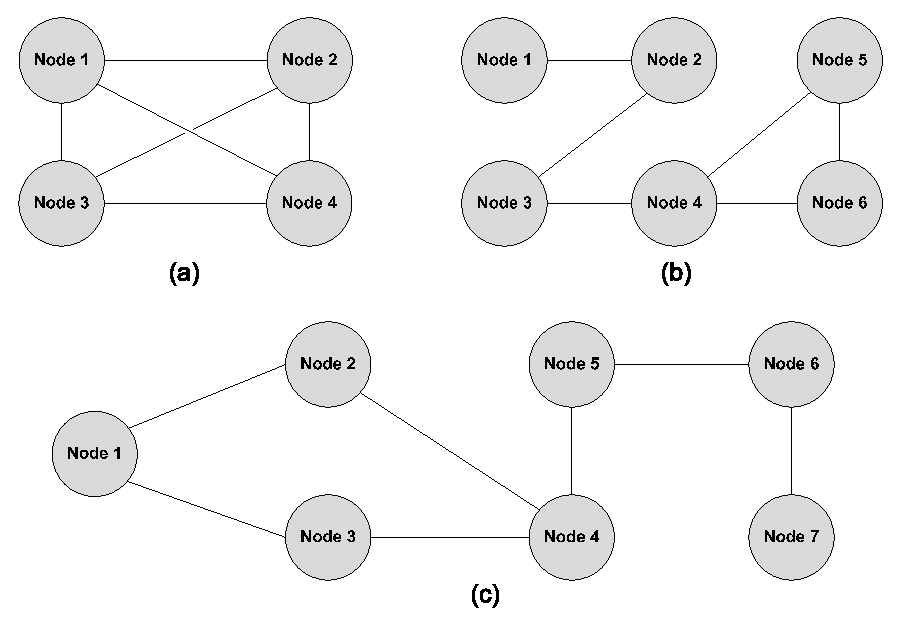
\includegraphics[scale=0.8]{dymo/graphics/topologies.eps}
\caption{Topologies to test the generated DYMO code}
\label{fig:topologies}
\end{figure}

To make sure that every part of the generated code at some point has been executed we have executed the generated DYMO code in the topologies shown in Fig.~\ref{fig:topologies}. In topology (a), node 1 makes a route request for node 4. This has the effect that all functions used to determine the usefulness of routing information is executed at least once. In topology (b), node 1 is requesting a route to node 6. This shows that the nodes are capable of establishing a route which consists of four hops. To further investigate the length of the routes we constructed topology (c), where node 1 is requesting a route to node 7. This test the part of the code that deals with the hop limit of a message. The shortest route between node 1 and node 7 has four intermediate nodes. When executing the protocol, where the messages contain a hop limit of four, the route could not be established. By increasing the hop limit to five the route was established through the four intermediate hops. Having all parts of the generated code executed with the expected outcome builds confidence in the correctness of the generated code.


